\chapter{Results}\label{chapter:results}

This chapter explains the evaluation methods used for evaluating the performance of machine learning models and presents the results.

\section{Evaluation Criteria} \label{sec:evaluationCriteria}

\subsection{Performance measures}
% Precision, Recall, Fscore
The performance measures \textit{Precision}, \textit{Recall} and \textit{F score} are used for calculating of performance of the machine learning models \textit{SSModel} and \textit{DSModel}.

For the task of protein-location relation extraction, a positive prediction is the one in which the machine learning model predicts a PL (protein-location) relation between a protein entity and a location entity. Similarly, a negative prediction is the one in which the machine learning model predicts that there is no relation between a protein entity and a location entity. 

A prediction can be classified into one of the following categories:


\begin{itemize}

\item \textit{True positive (tp)}: A prediction is said to be a true positive if it is a positive prediction (i.e., the entities are predicted to be related) and it matches an original relation in the corpus.

\item \textit{True negative (tn)}: A prediction is said to be a true negative if it is a negative prediction and the entities in the relation are also not related in the original corpus.

\item \textit{False positive (fp)}: A prediction is said to be a false positive if it is a positive prediction but the participating entities are not related in the original corpus.

\item \textit{False negative (fn)}: A prediction is said to be a false negative if it is a negative prediction but the participating entities are related in the original corpus.

\end{itemize}

\subsubsection*{\textit{Precision}}

Precision is the fraction of true predictions from all predictions and is given by:

$$
\textit{Precision} = \frac{tp}{tp+fp}
$$


\subsubsection*{\textit{Recall}}

Recall is the fraction of true predictions compared to original relations and is given by:

$$
\textit{Recall} = \frac{tp}{tp+fn}
$$

\subsubsection*{\textit{F score}}

F score, also called as F1 score, is the harmonic mean of precision and recall. It is given by:

$$
\textit{F score} = 2 * \frac{Precision * Recall}{Precision + Recall}
$$


\subsection{Evaluation mode - Non unique evaluation}

For a particular document in the corpus, it may happen that a protein is related to a location twice in the document at different places. In the non-unique evaluation mode, such repetitions are considered separately. A predicted relation is said to match with an original relation if and only if the text offsets of both protein and location entities in the predicted relation matches exactly with the text offsets of protein and location entities in the original relation respectively.


% Talk about unique relations here
\subsection{Evaluation mode -  Unique evaluation}

In the unique evaluation mode, a list of unique protein-location relations is made for every document in the corpus, notwithstanding the repetition of relations in the document. A predicted positive relation is said to match if and only if the predicted relation for the document is found in the list of unique relations for that document. If the predicted relation is not found in the list, it is either classified as a false positive or a true negative depending on whether it is a positive prediction or a negative prediction.

\section{Results for \textit{SSModel}}

This section presents the results for same sentence model (\textit{SSModel}). The results are initially discussed for the model trained on training data and evaluated on development data. All experimentation such as feature selection, hyperparameter search is performed with the development data. Once the the number of features to keep and the hyperparameter is fixed, the training model is used to evaluate the test data. The results on unseen test data are considered final results. All following subsections until subsection \ref{subsec:SSFinalRes} presents the results for a model trained on training data and evaluated on development data.

%After all experimentation, an additional model is training combining training and development data. Such a model is used to evaluate the test data and the results in such a way are considered much more robust.
 
\subsection{Initial results}

\begin{figure}
\centering
\begin{minipage}{.5\textwidth}
  \centering
  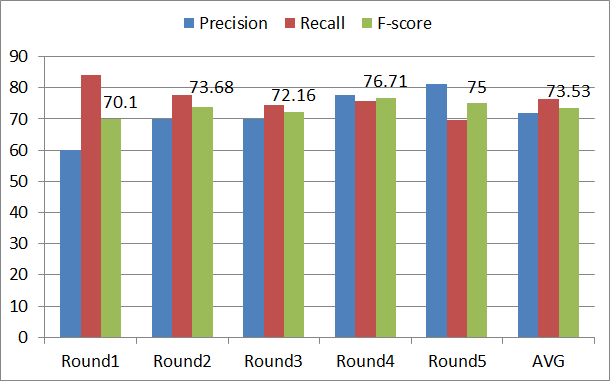
\includegraphics[width=.95\textwidth]{figures/SSInitialResultsNUniq.png}
  \caption{\textit{SSModel} non unique results}
  \label{fig:SS_NU_Initial}
\end{minipage}%
\begin{minipage}{.5\textwidth}
  \centering
  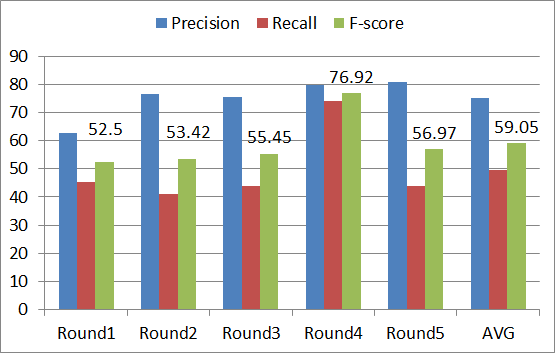
\includegraphics[width=.95\textwidth]{figures/SSInitialResultsUniq.png}
  \caption{\textit{SSModel} unique results}
  \label{fig:SS_U_Initial}
\end{minipage}
\end{figure}

As explained in the section \ref{sec:training}, 5-fold cross-validation is performed on the LocText corpus. For the details of cross-validation, refer to the section \ref{sec:training}. The primary evaluation results are shown in figures \ref{fig:SS_NU_Initial} and \ref{fig:SS_U_Initial}. Figure \ref{fig:SS_NU_Initial} shows the results of \textit{SSModel} using non unique evaluation method and fig. \ref{fig:SS_U_Initial} shows the results of \textit{SSModel} using unique evaluation method. The results are shown in terms of \textit{Precision}, \textit{Recall} and \textit{F score} for every round of cross validation and average performance is shown in the end. The \textit{F score} bars in the figures are also labeled with the actual value. Therefore, the non unique average \textit{F score} for \textit{SSModel} is 73.53 and unique average \textit{F score} for \textit{SSModel} is 59.05 as shown in the figures.

\subsubsection{Experimentation}

In order to make \textit{SSModel} robust and adaptable to other corpus, a lot of experimentation is carried out. Before the experimentation, every round of cross validation creates a model from around 30000 features on average. A lot of these features can be very specific to the LocText corpus and therefore, the efforts are made to discard unnecessary and redundant features. Following types of experiments are carried out:

\begin{itemize}

\item Leave One Out Analysis

\item Feature Weight Ranking

\item Information Gain Analysis

\end{itemize}

These experimentation methods are discussed in upcoming sections. This experimentation falls into the category of feature selection broadly discussed in the section \ref{sec:featSel}.

\subsection{Results after Leave One Out Analysis}

\begin{figure}
\centering
\begin{minipage}{.5\textwidth}
  \centering
  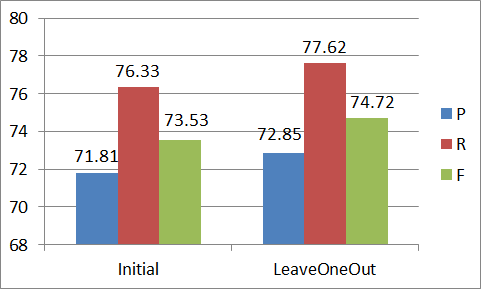
\includegraphics[width=.95\textwidth]{figures/LeaveOneOutNUniq.png}
  \caption{Non unique results comparison}
  \label{fig:LeaveOO_NU}
\end{minipage}%
\begin{minipage}{.5\textwidth}
  \centering
  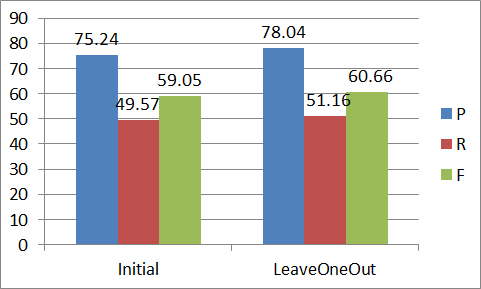
\includegraphics[width=.95\textwidth]{figures/LeaveOneOutUniq.png}
  \caption{Unique results comparison}
  \label{fig:LeaveOO_U}
\end{minipage}
\end{figure}

The theory behind Leave One Out approach is discussed in detail in the subsection \ref{subsec:LeaveOneOut}. To summarize this approach, the feature generators or functions that generates the features are greedily discarded to improve the performance of the model.

Figure \ref{fig:LeaveOO_NU} and \ref{fig:LeaveOO_U} shows the comparison between the results of initial model and after performing the LeaveOneOut experimentation.  The \textit{Precision}, \textit{Recall} and \textit{F score} are denoted by P, R and F respectively. Figure \ref{fig:LeaveOO_NU} shows the comparison using non-unique evaluation method and \ref{fig:LeaveOO_U} shows the comparison using unique evaluation mode. As shown in the figures, the average \textit{F score} increased from 73.53 to 74.72 for non-unique evaluation and from 59.05 to 60.66 for unique evaluation. In addition to the increase in the performance, the initial model used around 30900 features on average in every round of the cross validation. However, the model refined after LeaveOneOut experimentation uses 29000 features on average in every round, therefore reducing the number of features by 1900 for every round of the cross-validation.

\subsection{Results after Feature Weight Ranking}

The Feature Weight Ranking approach, discussed in detail in the subsection \ref{subsec:FWR}, uses the weights of the features for feature selection. The support vector machine model learns the weights for the features. These weights can be extracted from the learned model using a perl script \cite{svmlightonline}. 
 

\subsection{Results after Information Gain Analysis}

\subsection{Final Results}\label{subsec:SSFinalRes}

\section{Results for \textit{DSModel}}

\section{Results for CombinedModel}

\section{Assessment of Performance evaluation results}

%  Explain about statistical significance tests